
\chapter{Single-core Design}
\startcontents[chapters]
\printcontents[chapters]{}{1}{}
\noindent\\
While the majority of this report will focus on the multi-processing functionality of this project, it is important understand the design decisions of the single core that will be instantiated many times.

\section{Introduction}
\subsection{Design and Implementation}
The RISC core design is a traditional 5-stage processor (fetch, decode, execute, memory, write-back).

To satisfy \ref{cd:vendor}, the Verilog code will be self-contained in a single file. This reduces the hierarchical complexity and eases cross-vendor project set-up as only a single file is required to be included. 
A disadvantage with this single file approach is that some external Verilog verification tools that I plan to use, such as Verilator, do not currently support multiple Verilog modules (due to an unfixed bug) within a single file. 

\begin{figure}[H]
\centering 
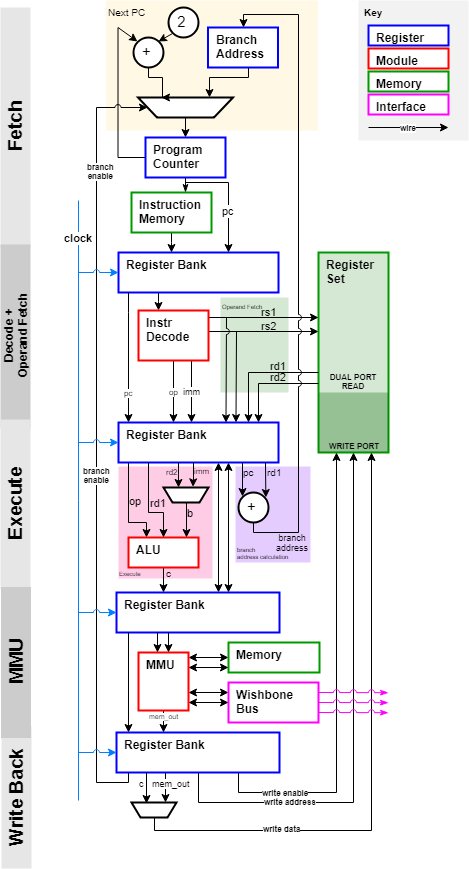
\includegraphics[width=10cm]{../img/risc}
\caption{Vmicro16 RISC 5-stage RTL diagram showing: instruction pipelining (data passed forward through clocked register banks at each stage); branch address calculation; ALU operand calculation (rd2 or imm); and program counter incrementing.}
\label{fig:risc}
\end{figure}

\subsection{Optimisations}
It is important in a multi-core design to

A small reduction in size within the single-core will result in substantial size reductions in 

\subsubsection{Instruction and Data Memory}
The design uses separate instruction and data memories similar to a Harvard architecture computer. This architecture was chosen due because I find it easier to implement.

\subsubsection{Register File}
To support design goal \ref{isa:regs}, the register set features a dual-port read and single-port write. This allows instructions to read 2 registers simultaneously for any instruction. The single-port write allows the instruction output to be written to the register file. 

\subsubsection{Pipelining}